\section{Simulation}

\begin{figure}[h]
\centering
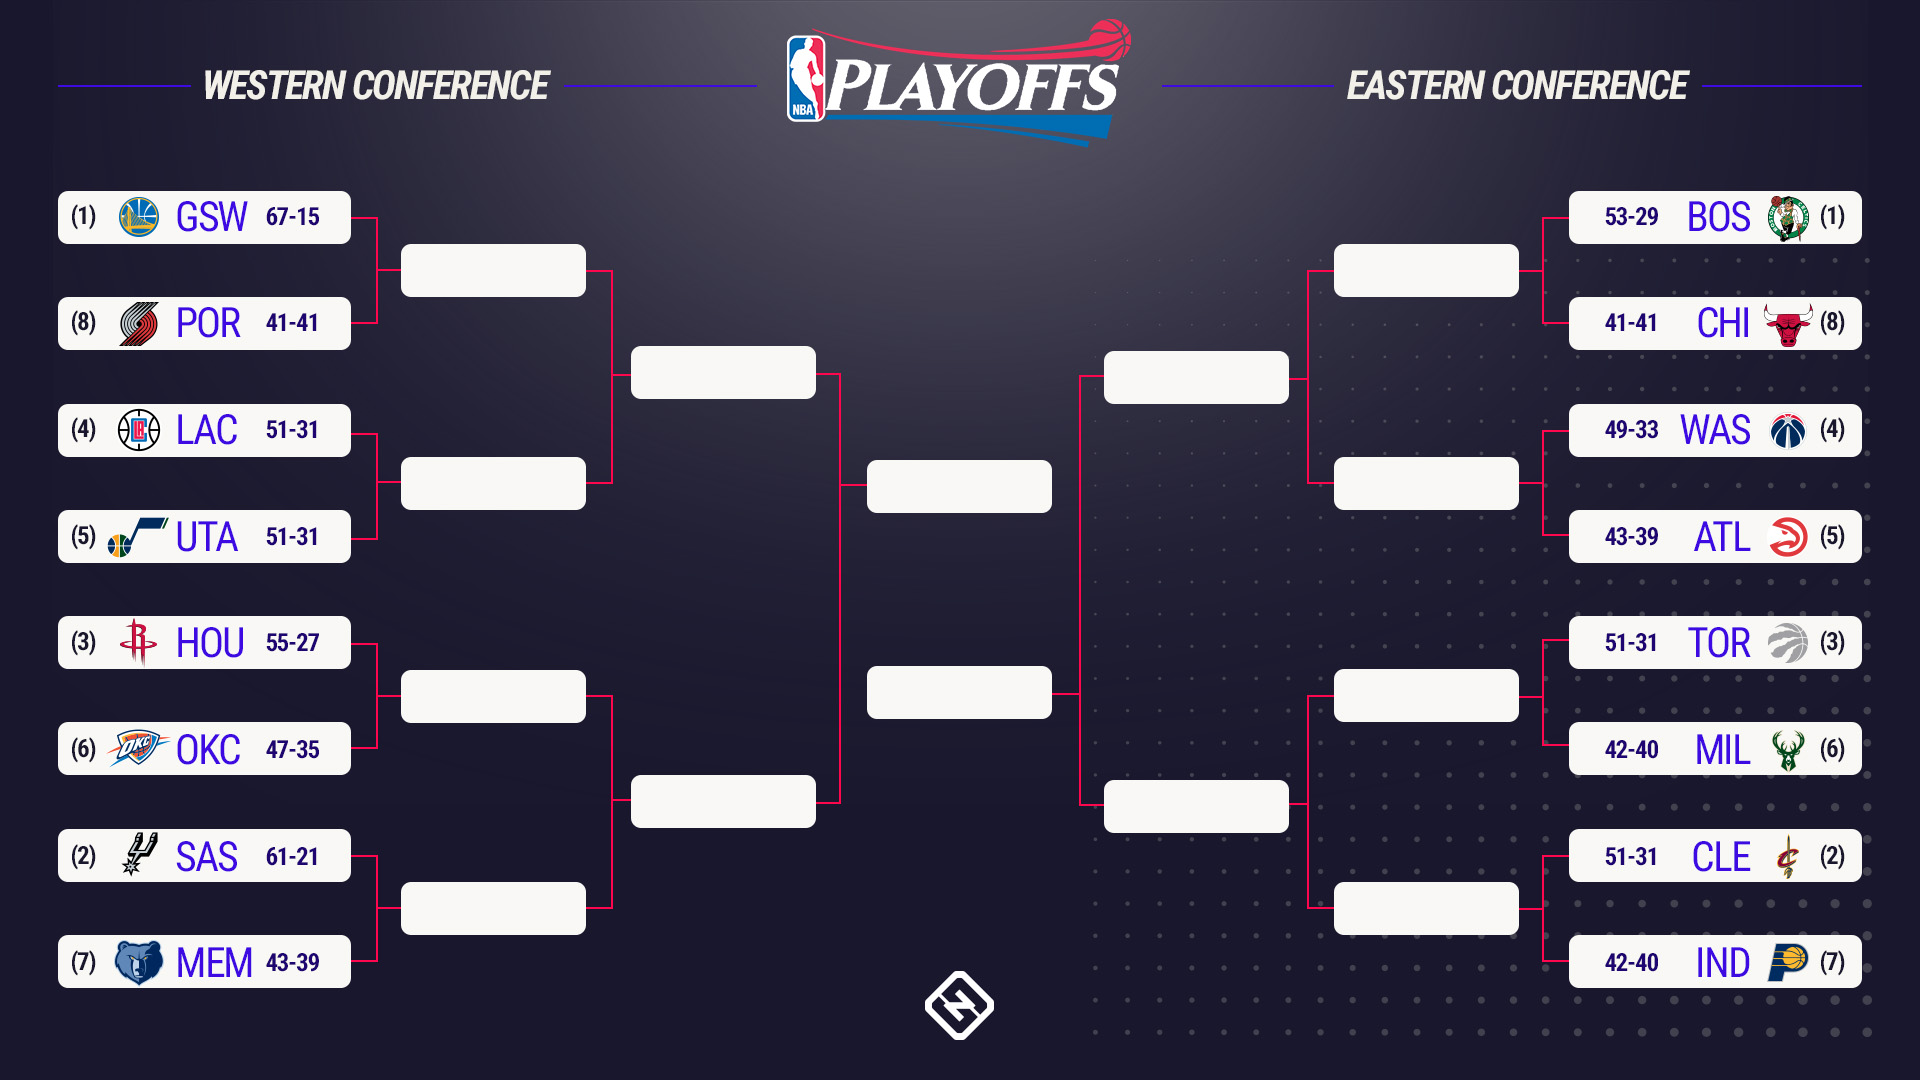
\includegraphics[width=\textwidth]{Format}
\end{figure}

The first round of the NBA playoffs, or conference quarterfinals, consists of 
four match-ups in each conference based on the seedings (1–8, 2–7, 3–6, and 4–5).
The four winners advance to the second round, or conference semifinals, with a 
match-up between the 1–8 and 4–5 winners and a match-up between the 2–7 and 3–6
winners. The two winners advance to the third round, or conference finals.
The winner from each conference will advance to the final round, or the NBA Finals.

According the NBA rules, all rounds are $best-of-seven$ series. Series are played
in a 2-2-1-1-1 format, meaning the team with home-court advantage hosts games
1, 2, 5 and 7, while their opponent hosts games 3, 4, and 6, with games 5-7 
being played if needed.

Based on our model, given two teams Team A and Team B, we will have two
probabilities based on whether Team A plays in the home filed.
According to the schedule and playoff rules, we simulated the result for 
each game and predicted the winners for each layer, from the first round:
8 teams in both Western and Eastern Conference, to the final layer: 
only 1 team left in both Conference and fight for the championship. 

Importantly, in each layer, we can update our features and wining probabilities
by incorporating the most up-to-date data. And as the real games go on, we can
correct the winner of each round and continue the simulation process. 


